\documentclass[11pt]{article}
%基于北京航空航天大学仪器科学与光电工程学院实验报告及课程报告排版得来,类似于毕业论文排版格式
%后续将更新毕业论文排版格式
\usepackage{graphicx,float}%使用图的宏包,使用图的浮动体宏包,引入参数H使图像紧跟当前文字
\usepackage{caption} %使用图表标题的宏包
\usepackage[colorlinks=true,pdfstartview=FitH,%
linkcolor=black,anchorcolor=violet,citecolor=magenta]{hyperref}%加载hyperref宏包,使用超链接
\usepackage{setspace}%用于设置行间距列间距等命令的宏包
\usepackage{array}%设置列表高度宽度的宏包
\usepackage{zhnumber}%使用中文数字编号的宏包
\usepackage{titlesec,titletoc}%使用标题自定义形式的宏包和使用目录自定义形式的宏包
\usepackage{siunitx}%物理学单位宏包
\usepackage{tabularx}%让表格宽度等于页面宽度
\usepackage{makecell}%单个表格单元调整的宏包
\usepackage{subfigure} %%使用子图的宏包
\usepackage[backend=biber,bibstyle=gb7714-1987,%nature,%%加载biblatex宏包,使用参考文献
citestyle=gb7714-1987%,backref=true%%其中后端backend使用biber
,url=false
]{biblatex}%标注(引用)样式citestyle,著录样式bibstyle都采用gb7714-2015样式
% \usepackage{pgfplots}%类似tikz的一个画图库,主要画统计图
\usepackage{customFont}%自行编写的字体命令库,基于CJK宏包
\usepackage{bh_style}%自行编写的风格文件,基于使用习惯和格式要求
\usepackage{math_formulate}%自行编写的数学公式命令库,基于amsmath宏包
\usepackage{picture}%集成图形绘制库,主要包括了tikz和pgfplots两大主流宏包
% \usepackage[lite,subscriptcorrection,slantedGreek,nofontinfo]{mtpro2}%使用mathtimepro2商业字体作为数学环境,并不推荐

%biblatex宏包的参考文献数据源加载方式,注意book.bib应当与.tex文件在同一目录下,不然有可能会报错
\addbibresource[location=local]{book.bib}
% % \bibliographystyle{gbt7714-numerical}
%%% 下面的命令重定义页面边距,使其符合中文刊物习惯 %%%%
% \addtolength{\topmargin}{2.5cm}
\setlength{\oddsidemargin}{0.63cm}  % 3.17cm - 1 inch
\setlength{\evensidemargin}{\oddsidemargin}
% \setlength{\textwidth}{14.66cm}
% \setlength{\textheight}{24.00cm}    % 24.62

\graphicspath{{E:/Code/git/Latex-Tempulate/fig}}

\begin{document}
{
\pagestyle{empty}
\begin{figure}
  
\includegraphics{title.jpg}
\end{figure}
\begin{center}

  \begin{figure}[h]

    \centering
    
\includegraphics[]{title.png}\par
    \vspace{4em}
    \large{\yihao\lishu{2022-2023学年第一学期}}
    \vspace{6em}
  \end{figure}

  \large{\erhao\lishu{《基于Latex的实验报告撰写与排版》}}\par
  \large{\erhao\lishu{ 课程实验报告  }}
  \vspace{8em}

  \begin{spacing}{2.0}
    \begin{tabular}{cc}


      {\xiaoerhao\lishu{班\quad \quad 级}} & {\heiti{\dlmu{123456班}}}   \\
      {\xiaoerhao\lishu{学\quad \quad 号}} & {\heiti{\dlmu{12345678} }} \\
      {\xiaoerhao\lishu{姓\quad \quad 名}} & {\heiti{\dlmu{Tschen} }}   \\
      {\xiaoerhao\lishu{日\quad \quad 期}} & {\heiti{\dlmu{\today} } }  \\
    \end{tabular}
  \end{spacing}
\end{center}
\thispagestyle{empty}
}


\newpage
%手动分页
\pagenumbering{roman}
%摘要
\begin{abstract}


  本次课程设计综合运用了光电探测技术、成像技术、红外成像技术相关的知识,进行了给定要求下的红外成像系统设计(含光学设计),对经过大气消光作用后的目标辐射、成像元件NETD以及识别准则进行了分析和陈述,最后进行了光学系统的设计并检验了其孔径和视场要求,除所设计的系统尺寸较大(约32cm)以外,其他要求均符合预期。
\end{abstract}
%目录

\newpage
\setcounter{tocdepth}{3}
%设定目录深度                      
\tableofcontents
%列出目录




\newpage

\pagenumbering{arabic}
\setcounter{page}{1}
\section{实验目的}
\begin{enumerate}
  \item 熟悉大气对光电探测影响的分析方法;
  \item 熟悉红外热像仪性能的分析方法;
  \item 熟悉红外热像仪光学系统的设计方法;
  \item 了解影响热像仪空间分辨能力的因素(选做)。
\end{enumerate}

\section{题目要求}
\subsection{红外成像芯片参数}
利用表中的红外成像芯片设计一款红外热像仪。\par
\begin{table}[H]
  \centering
  \caption{红外成像芯片参数表}
  \renewcommand{\arraystretch}{1.5}
  \label{table:红外成像芯片参数}
  \begin{tabular}{|m{0.3\textwidth}<{\centering}|m{0.3\textwidth}<{\centering}|m{0.3\textwidth}<{\raggedright\arraybackslash}|}
    \hline
    项目     & 参数                               & \makecell*[c]{备注}                                       \\\hline
    探测器类型  & 非制冷氧化钒                           &                                                         \\\hline
    响应波段   & $8\sim 14\unit{\um}$             &                                                         \\\hline
    红外分辨率  & $ 640 \times 480$                &                                                         \\\hline
    成像单元尺寸 & $12\unit{\um}\times12\unit{\um}$ &                                                         \\\hline
    NETD   & $50\unit{mK}@F1.0/50\unit{\Hz}$  & {50mK表示噪声等效温差为50mK,F1.0指相对孔径为1.0,50Hz表示此参数是帧频50Hz下测得的 } \\\hline
    帧频     & $50\unit{\Hz}$                   &                                                         \\\hline
  \end{tabular}
\end{table}

\subsection{红外成像系统性能指标}
\begin{itemize}
  \item 目标参数:大小$3\unit{\m}\times2\unit{\m}$、目标表面温度320K、背景温度300K;
  \item 大气模型:考虑USSA1976 大气模型;
  \item 天气条件:气象能见度20km;
  \item 探测距离:>10km(水平);
  \item 识别距离:>2km(水平)(不考虑大气传输产生的图像模糊);
\end{itemize}
\section{要点提醒}
对于所有的处理过程都要给出理论依据,不能只给出处理结果,要写成正式的课程设计报告。\par
本课程设计需要考虑以下几个方面的问题:
\begin{enumerate}
  \item 大气对光传输的影响(采用USSA1976 大气模型,大气透过率的理论计算  依据,可以利用Modtran 软件计算大气透过率);
  \item 目标的探测与识别问题(不同辨别等级的准则、NETD 的修正、探测和识别距离的计算方法);
  \item 光学系统的设计(光学系统参数的计算:孔径、焦距、视场、光阑等)。
\end{enumerate}
\section{系统设计分析}
\subsection{目标发光情况}
将目标当作黑体,计算其辐射的情况:\par
辐射辐亮度随波长的关系:
\begin{equation}
  L_{O\lambda}(T)=\frac{2\pi hc^2}{\lambda^5 \rectbrac{e^{C_2/(\lambda T)}-1}}=\frac{C_1}{\pi\lambda^5}\frac{1}{e^{C_2/(\lambda T)}-1}
  \label{forem:普朗克公式,辐亮度,波长}
\end{equation}

辐射辐亮度随波数的关系:
\begin{equation}
  L_{O\nu}(T)=\frac{2\pi hc^2\nu^3}{e^{C_2\nu/T}-1}=\frac{C_1\nu^3}{\pi}\frac{1}{e^{C_2\nu/T}-1}
  \label{forem:普朗克公式,辐亮度,波数}
\end{equation}


\begin{figure}[H]
  \centering
  \subfigure[目标辐射体辐亮度与波长的关系]{
    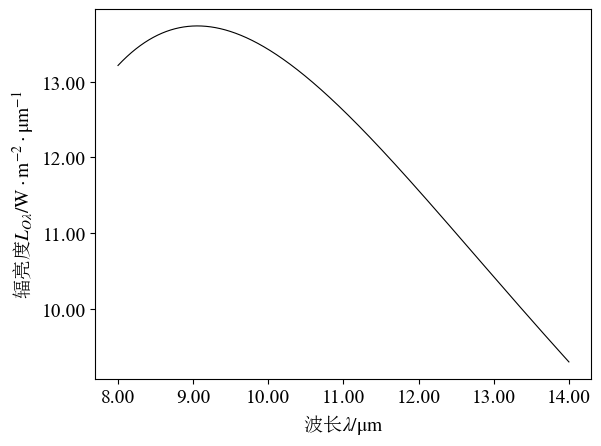
\includegraphics[width=0.45\textwidth]{普朗克公式,辐亮度,波长.png}
    \label{subfig:普朗克公式,辐亮度,波长}
  }
  \centering
  \subfigure[目标辐射体辐亮度与波数的关系]{
    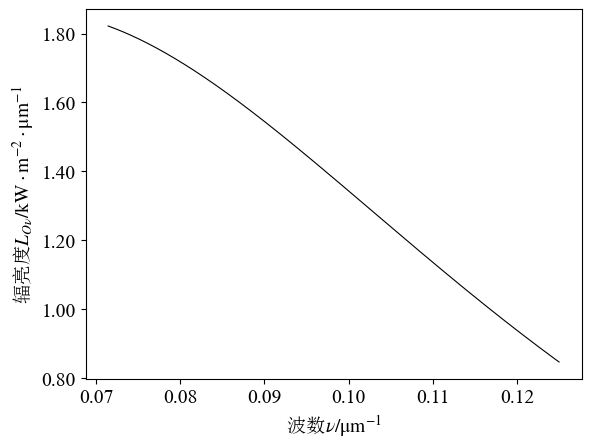
\includegraphics[width=0.45\textwidth]{普朗克公式,辐亮度,波数.png}
    \label{subfig:普朗克公式,辐亮度,波数}
  }
  \caption{目标辐射体亮度}
  \label{fig:普朗克公式}
\end{figure}
由于红外成像芯片的敏感波段是$8\sim14\unit{\um}$,因此着重考查这部分的辐射情况。代入第一辐射常数$C_1=2\pi c^2h=3.7413\times 10^8\unit{\W\cdot \um^4/\m^2}$和第二辐射常数$C_2=hc/K=1.4388\times 10^4\unit{\um\cdot \K}$以及目标辐射体的温度$T=320\unit{\K}$,可知黑体的辐射情况如图\ref{fig:普朗克公式}所示。\par
同理,根据维恩位移公式可得:
\begin{equation}
  \lambda_m=\frac{a}{T}
  \label{forem:维恩位移公式}
\end{equation}

其中:$a=\rm 2.897\times 10^{-3}m\cdot K$是维恩常数。\par
因此峰值辐射波长为:$\displaystyle\lambda_m=\rm \frac{2.897\times 10^{-3}}{320}=9.053\times 10^{-6}\unit{\m}=9.053\unit{\um}$。\par
总辐射出射度可以使用对全波长积分,即有:
\begin{equation}
  M_O(T)=\int_0^\infty M_{O\lambda}(T)d\lambda=\frac{C_1\pi
    ^4T^4}{15C_2^4}=\sigma T^4
  \label{forem:总辐出度公式}
\end{equation}

其中:$\sigma=5.67\times 10^{-8} \unit{\J\cdot\m^{-2}\cdot \s^{-1}\cdot \K^{-4}}$是斯蒂芬-玻尔兹曼常数。\par
因此总辐射强度为:$M_O(T)=594.54\unit{\W\cdot \m^{-2}}$。\par
最大辐射出射度:
\begin{equation}
  M_{O\lambda_m}(T)=BT^5
  \label{forem:最大辐出度公式}
\end{equation}

式中,$B= 1.2862\times 10^{-11}\unit{\W\cdot \m^{-2}\cdot \um^{-1}\cdot \K^{-5}}$。\par
因此最大辐射出射度为:$M_{O\lambda_m}(T)=0.132\unit{\MW\cdot \m^{-2}\cdot \um^{-1}}$。
\subsection{大气对光传输的影响分析}
一般来说,根据课堂讲义\cite*{hand_up}和文献\cite*{optical_electrical_photography}知,可以通过以下的十二个步骤人工查表计算,如:\par
第一步,查表知海平面1\unit{\km}大气中,已知相对湿度$H_r$时的可降水分厘米数;\par
第二步:求在已知相对湿度$H_r$情况下,1km大气中的可降水分毫米数;\par
第三步:计算水分高度修正路径长度: $ \displaystyle L_0({\rm H_2O})  =L\times e^{-0.05938z} $;\par
第四步:计算沿路径长度水分含量;\par
第五步:查表求得与水气相关的大气透过率$\tau_{\rm H_2O}$,必要时,使用函数内插;\par
第六步:计算$\rm CO_2$的高程修正路径长度:$\displaystyle L_0({\rm CO_2})  =L\times e^{-0.178z}  $;\par
第七步:查表求得与$\rm CO_2$相关的大气透过率$\tau_{\rm CO_2}$;\par
第八步:根据大气能见度,计算气溶胶衰减系数,其中大气的密度可按下式求得:$\displaystyle\rho(z)  =\rho_0\times e^{-\frac{g}{RT}(z-z_0)} $,此处的R是气体常数,值为$287.06\unit{\J\cdot\kg^{-1}\cdot\K^{-1}}$;\par
第九步:计算气溶胶对大气透过率的贡献:
$\displaystyle\tau_{\rm asl}=e^{-\frac{3.912}{R_v}R}$;\par
第十步:根据经验公式计算雨的散射系数$\displaystyle\beta_{\rm rain}=0.248V^{h}$,式中$h$为降雨速率;\par
第十一步:计算雨对大气透过率的贡献,根据波盖耳定律:$\displaystyle\tau_{\rm rain} =e^{-\beta_{\rm rain}\rho s}$;\par
第十二步:计算总的大气透过率;\par
采用USSA1976大气模型,因此首先需要使用MODTRAN软件对大气透过率进行仿真计算,其大气模式的吸收曲线如下图\ref{fig:USSA1976大气模型吸收曲线,水平路径12km,海拔1km}所示:
\begin{figure}[H]
  \centering
  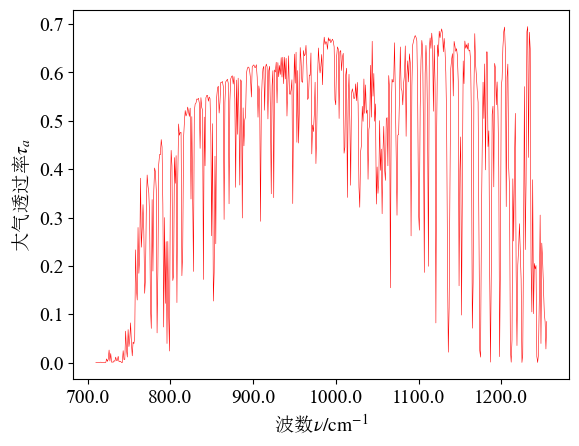
\includegraphics[width=0.8\textwidth]{大气透过率,波数,12km.PNG}
  \caption{USSA1976大气模型吸收曲线,水平路径12km,海拔1km}
  \label{fig:USSA1976大气模型吸收曲线,水平路径12km,海拔1km}
\end{figure}
\par
按波数表达的目标辐射体辐亮度在经过大气消光作用后到达探测器物镜的图线如图\ref{fig:辐亮度,已消光,12km}所示:
\begin{figure}[H]
  \centering
  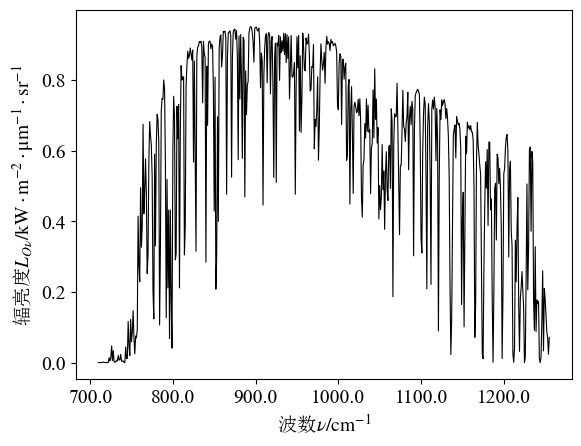
\includegraphics[width=0.8\textwidth]{普朗克公式,辐亮度,波数,已消光,12km.PNG}
  \caption{经过12km传播大气消光作用的辐亮度}
  \label{fig:辐亮度,已消光,12km}
\end{figure}
\par
如果取峰值波数$\nu_m=1104.6\unit{\cm^{-1}}$处的辐亮度,其经过消光作用后得到的值为$L_{O\nu_m}=172\unit{\W\cdot \m^{-2}\cdot \um^{-1}\cdot sr^{-1}}$,并不是消光之后的最大亮度,查阅消光后辐亮度的列表,可得最大辐亮度应该是波数$\nu_0=849\unit{\cm^{-1}}$处的辐亮度,其经过消光作用后得到的值为$L_{O\nu_0}=978.3\unit{\W\cdot \m^{-2}\cdot \um^{-1}\cdot sr^{-1}}$
\subsection{目标的探测与识别分析}
\subsubsection{不同辨别等级的准则}
首先根据Johnson准则,对识别和探测所需要的条纹数进行界定,得到表\ref{table:Johnson准则}如下:
\begin{table}[H]
  \renewcommand{\arraystretch}{1.5}
  \centering
  \caption{工业上采用的Johnson准则辨识标准}
  \label{table:Johnson准则}
  \begin{tabularx}{\textwidth}{|c|>{\centering}X|c|}
    \hline
    辨别等级 & 定义                 & 最小尺寸上的周期数 \\\hline
    探测   & 存在一个目标,把目标从背景中区别出来 & 1         \\\hline
    识别   & 识别出目标属于哪一个类别       & 4         \\\hline
    辨别   & 认出目标,并能足够清晰地确定其类型  & 8         \\\hline
  \end{tabularx}
\end{table}
\subsubsection{NETD的修正}
假设目标辐射体在探测器上的成像尺寸小于探测器单元的尺寸,则不妨设目标的大小为$\alpha\times\beta$,探测单元的大小为$a\times b$,像的大小为$a'\times b'$,则利用修正公式$\displaystyle \mathrm{NETD}'=\frac{ab}{a'b'}\times\mathrm{NETD}$。\par
解得修正系数为$\displaystyle k=\frac{ab}{a'b'}=\frac{\Delta T}{\mathrm{NETD}}=\frac{20}{50\times10^{-3}}=400$,因此目标像在探测平面上的大小为$\displaystyle a'b'=\frac{ab}{k}=\frac{12\times12}{400}=0.36\unit{\um^2}$。\par
由于目标大小为$3\unit{\m}\times2\unit{\m}$,因此根据比例关系:$\displaystyle\frac{a'}{b'}=\frac{3}{2}$,解得:
\begin{align*}
  \left\{
  \begin{aligned}
    a' & =1.5\times\sqrt{0.24}=0.7348\unit{\um} \\
    b' & =\sqrt{0.24}=0.4899\unit{\um}
  \end{aligned}
  \right.
\end{align*}
\subsubsection{探测和识别距离的计算}
假设红外成像仪的焦距为$f_0'$,探测距离为$L_d$,根据几何光学成像条件,在符号设计要求的前提下,其临界条件应当满足:
\begin{equation*}
  \frac{f_0'}{L_d}=\frac{a'}{\alpha}\implies f_0'=\frac{a'}{\alpha}\times L_d=\frac{0.7348\times10^{-6}}{3}\times 10\times10^3=2.45\unit{\mm}
\end{equation*}
而Johnson准则只要求检测到一个周期就可以了,因此上式不用再作修正,计算得到的结果就 是焦距的临界值,而要求探测距离$L_d>10\unit{\km}$,即焦距应当比这个值更大,$f_0'>2.45\unit{\mm}$。\par
根据Johnson准则,识别目标辐射体应当在目标的最小尺寸上分辨出4个周期,因此对应目标像的大小应该至少覆盖8个像素,即探测器所能测量的最小尺寸,因此,如果设能够识别的目标像的大小为$a''\times b''$,其应该满足:
\begin{align*}
  \left\{
  \begin{aligned}
    a'' \geq a'\times8=96\unit{\um} \\
    b''\geq b'\times8=96\unit{\um}
  \end{aligned}
  \right.
\end{align*}\par
由于目标像的宽度尺寸更小,因此需要保证在宽度上能够识别,则长度应该按比例计算为$\displaystyle a''=1.5\times b''=144\unit{\um}$。
同理,可以利用识别条件,计算得到有关成像仪焦距的另一个约束条件:
\begin{align*}
  \frac{f_0'}{L_c}=\frac{a''}{\alpha}\implies f_0'=\frac{a''}{\alpha}\times L_c=\frac{144\times10^{-6}}{3}\times2\times10^3=96\unit{\mm}
\end{align*}\par
实际的焦距应该大于这个临界值,即$f_0'>96\unit{\mm}$。
\section{光学设计}

本红外成像光学系统,由于是对远距离物体成像,所以在本质上是一个照相系统,根据孔径的关系,再判断需不需要在照相系统的物方增加一个望远系统。考虑以上条件,本系统应至少一个提供光焦度的会聚透镜$f_3'=f_0'$,可能含有两个会聚透镜$f_1'$和$f_2'$,以及红外成像芯片安装在会聚透镜$f_3'$的焦平面上,除此以外,目前还有以下约束条件:
\begin{enumerate}
  \item 系统的总焦距为$f_0'>96\unit{\mm}$;
  \item 系统的相对孔径为$F=1.0$;
  \item 系统的孔径光阑是望远镜的物镜;
  \item 系统的视场光阑是望远镜的分划板;
  \item 系统的渐晕光阑是望远镜的目镜;
  \item 系统的入瞳距为0;
\end{enumerate}

\subsection{照相系统设计}
\begin{figure}[H]
  \centering
  \begin{tikzpicture}
    \coordinate (O) at (0,0);
    \coordinate (A) at (14,0);
    %三个透镜的光心
    \coordinate [label=below:$H_2$](F2) at (7,0);
    %CCD屏的光心
    \coordinate [label=below:成像芯片](CCD) at (12.2,-1);
    %主光轴
    \draw [-{Stealth}] (O) -- (A);
    %画照相系统
    \draw[] (F2) ellipse [x radius=0.2cm,y radius=2cm];
    \draw (CCD) rectangle (11.8,1) ;
    %光学参数
    \coordinate [label=below:$F_2$] (F2_l) at (2.2,0);
    \coordinate [label=above:$F_2'$] (F2_r) at (11.8,0);
    \filldraw (F2_l) circle [radius=0.6mm];
    \filldraw (F2_r) circle [radius=0.6mm];
  \end{tikzpicture}
  \caption{仅含一个物镜的红外成像仪的光学系统设计光路}
  \label{fig:红外成像仪,一个物镜}
\end{figure}
不考虑引入望远系统,只考虑照相系统。由于照相系统物镜相对孔径为$\displaystyle\frac{D_3}{f_3'}=1.0$,因此照相系统的入瞳,即是这里的物镜框$H_3$的尺寸$D_3$应该等于其焦距$f_3'=100\unit{\mm}$,红外成像芯片位于照相物镜的焦平面上,查工程光学设计手册\cite*{optical_design}中照相物镜的参数列表可知,最接近成像要求入瞳直径的物镜参数如下表所示:
\begin{table}[H]
  \renewcommand{\arraystretch}{1.5}
  \centering
  \caption{满足相对孔径要求的照相物镜参数列表}
  \label{table:照相物镜参数列表}
  \begin{tabularx}{\textwidth}{|c|>{\centering}X|>{\centering}X|c|}
    \hline
    标准值序号 & 焦距$f'$           & 相对孔径$D/f'$ & 入瞳直径$D$            \\\hline
    1     & $500\unit{\mm}$  & $1:4.5  $  & $111.1\unit{\mm}$  \\\hline
    2     & $600\unit{\mm}$  & $1:5.6  $  & $107.14\unit{\mm}$ \\\hline
    3     & $1200\unit{\mm}$ & $1:11  $   & $109.09\unit{\mm}$ \\\hline
  \end{tabularx}
\end{table}
\par
可见单独使用任意一个照相物镜都不满足相对孔径$F=1.0$的要求,因此必须在原物镜后面或者前面再增加一组放大镜,以构成远距型光路,使系统的等效焦距得以缩小,从而达到设计要求。
\begin{figure}[H]
  \centering
  \begin{tikzpicture}
    \coordinate (O) at (0,0);
    \coordinate (A) at (15,0);
    %三个透镜的光心
    \coordinate [label=below:$H_1$](F1) at (7,0);
    \coordinate [label=below:$H_2$](F2) at (10,0);
    %CCD屏的光心
    \coordinate [label=below:成像芯片](CCD) at (12.2,-1);
    %主光轴
    \draw [-{Stealth}] (O) -- (A);
    %画照相系统
    \draw[] (F1) ellipse [x radius=0.2cm,y radius=2cm];
    \draw[] (F2) ellipse [x radius=0.2cm,y radius=2cm];
    \draw (CCD) rectangle (11.8,1) ;
    %光学参数
    \coordinate [label=below:$F_1$] (F1_l) at (1.5,0);
    \coordinate [label=above:$F_1'$] (F1_r) at (12.5,0);
    \coordinate [label=below:$F_2$] (F2_l) at (6,0);
    \coordinate [label=above:$F_2'$] (F2_r) at (14,0);
    \filldraw (F1_l) circle [radius=0.6mm];
    \filldraw (F1_r) circle [radius=0
        .6mm];
    \filldraw (F2_l) circle [radius=0.6mm];
    \filldraw (F2_r) circle [radius=0.6mm];
  \end{tikzpicture}
  \caption{由两组透镜组成的物镜的红外成像仪的光学系统设计光路}
  \label{fig:红外成像仪,两个物镜}
\end{figure}
\par
即使新增加放大镜,如果能保证其在原照相物镜的物方空间的虚物尺寸大于物镜入瞳,整个照相系统的孔径光阑仍然是原照相物镜的入瞳$D$。如考虑兼顾最小尺寸,选取表\ref{table:照相物镜参数列表}中第2行的数据,则需要将整个系统的等效焦距缩短至$107.14\unit{\mm}$。\par
候选的放大镜的焦距为$150\unit{\mm}$,相对孔径$D/f'=1:1.4$,以此可求得放大镜的入瞳直径为$107.14\unit{\mm}$。设$H_1H_2=\Delta l_1$,$H_2$到成像芯片的距离为像距$l_2'$,假设一束平行光轴的光线从整个系统的物方入射,经两个透镜偏折后,其最终会聚于成像芯片的正中心,如下图所示:
\begin{figure}[H]
  \centering
  \begin{tikzpicture}
    \coordinate (O) at (0,0);
    \coordinate (A) at (15,0);
    %三个透镜的光心
    \coordinate [label=below:$H_1$](F1) at (7,0);
    \coordinate [label=below:$H_2$](F2) at (10,0);
    %CCD屏的光心
    \coordinate [label=below:成像芯片](CCD) at (12.2,-1);
    %主光轴
    \draw [-{Stealth}] (O) -- (A);
    %画照相系统
    \draw[] (F1) ellipse [x radius=0.2cm,y radius=2cm];
    \draw[] (F2) ellipse [x radius=0.2cm,y radius=2cm];
    \draw (CCD) rectangle (11.8,1) ;
    %光学参数
    \coordinate [label=below:$F_1$] (F1_l) at (1.5,0);
    \coordinate [label=above:$F_1'$] (F1_r) at (12.5,0);
    \coordinate [label=below:$F_2$] (F2_l) at (6,0);
    \coordinate [label=above:$F_2'$] (F2_r) at (14,0);
    \filldraw (F1_l) circle [radius=0.6mm];
    \filldraw (F1_r) circle [radius=0
        .6mm];
    \filldraw (F2_l) circle [radius=0.6mm];
    \filldraw (F2_r) circle [radius=0.6mm];
    %画一个光路
    \draw[line width=0.8pt,arrows = {-Stealth[inset=0pt, length=10pt, angle'=30]},red] (0,2) -- (4,2);
    \draw[line width=0.8pt,red] (3,2) -- (7,2) -- (10,0.909) -- (11.8,0);
    \draw[line width=0.8pt,red,dashed] (7,2) -- (7.84,2)--(10,0.909);
    \draw[line width=0.8pt,red,dashed] (7.84,2) -- (7.84,0)node[below,black]{$H'$};
    %画尺寸标注
    \begin{scope}[>={Stealth[inset=0pt, length=5pt, angle'=30]}]
      \draw[] (7.833,-.6) -- (7.833,-2.2);
      \draw[|<->|] (7,-2.2) --node[midway,above]{$l_H'$} (7.84,-2.2);
      \draw[|<->|] (7,-2.6) --node[midway,above]{$\Delta l$} (10,-2.6);
      \draw[|<->|] (10,-2.6) --node[midway,above]{$l_2'$} (11.8,-2.6);
    \end{scope}
  \end{tikzpicture}
  \caption{由两组透镜组成的物镜的红外成像仪的光学系统设计光路}
  \label{fig:红外成像仪,两个物镜,有光路}
\end{figure}
\par
根据透镜成像的高斯公式\cite*{optical_engineer}:
\begin{align}
  -\frac{1}{l_1}+\frac{1}{l_1'}=\frac{1}{f_1'} \\
  -\frac{1}{l_2}+\frac{1}{l_2'}=\frac{1}{f_2'}
  \label{forem:凸透镜成像的高斯公式}
\end{align}
\par
其中,下标为1的代表透镜$H_1$的物方截距、像方截距和焦距,下标为2的代表透镜$H_2$的物方截距、像方截距和焦距,暂设$\Delta l+l_2'=250\unit{\mm}$,则可得$l_2'=250-\Delta l$,$l_1\rightarrow-\infty$。转镜公式为:
\begin{equation*}
  l_1'-\Delta l=l_2
\end{equation*}
\par
联立以上各式可解得:
\begin{align}
  \Delta l^2-850\Delta l+97500=0\implies
  \left\{
  \begin{aligned}
    \Delta l & =136.69\unit{\mm} \\
    l_2'     & =113.31\unit{\mm}
  \end{aligned}
  \right.
  \label{forem:两个透镜,照相系统}
\end{align}
\par
解算其等效主点$H'$,设入射光线在第一面透镜上的投影高度为$h_1$,在第二面上的投影高度为$h_2$:
\begin{align*}
  \left.
  \begin{aligned}
    \frac{h_1}{h_2}=\frac{f_1'}{f_1'-\Delta l} \\
    \frac{h_2}{l_2'}=\frac{h_1}{\Delta l+l_2'-l_H'}
  \end{aligned}
  \right\}\implies l_H'=103.26\unit{\mm}
\end{align*}
\par
等效的焦距$f'=\Delta l+l_2'-l_H'=146.74\unit{\mm}$,这个等效的焦距在长度上满足题目设计要求,在相对孔径上稍微大了一点,因此,考虑调整以上布置使之符合相对孔径的设计要求。\par
设$\Delta l+l_2'=L$,公式\ref{forem:凸透镜成像的高斯公式}仍然成立,求主面的公式也成立,这里归纳在一起,如下列所示:
\begin{align}
  \begin{aligned}
    -\frac{1}{l_1}+\frac{1}{l_1'} & =\frac{1}{f_1'}                 \\
    -\frac{1}{l_2}+\frac{1}{l_2'} & =\frac{1}{f_2'}                 \\
    l_1'-\Delta l                 & =l_2                            \\
    \frac{h_1}{h_2}               & =\frac{f_1'}{f_1'-\Delta l}     \\
    \frac{h_2}{l_2'}              & =\frac{h_1}{\Delta l+l_2'-l_H'} \\
    \Delta l+l_2'                 & =L                              \\
    f'=\Delta l+l_2'-l_H'         & =107.14\unit{\mm}
  \end{aligned}
  \label{forem:完整的双透镜成像求解式}
\end{align}
\par 解得$l_2'=123.215\unit{\mm}$,$\Delta l=-90.02\unit{\mm}$,并不符合物理模型,因此需要将两个透镜的位置对换,再考察其安装,这里,沿用\ref{forem:完整的双透镜成像求解式}的算式,将其中的$f_1'=150\unit{\mm}$,$f_2'=600\unit{\mm}$代入式中,再次求解上述方程组,解得:$l_2'=173.27\unit{\mm}$,$\Delta l=-90.02\unit{\mm}$
也不成立,说明仅用这两个透镜构成的光学系统不满足实际需要,因此需要进一步调整。为保证孔径光阑不发生改变,再引入一个相同的放大透镜,与原放大镜构成一个等效透镜,这个等效透镜的主平面距离为$l_{H_2H_2'}$,焦距为$f_2'$,等效透镜的物方主平面距离照相物镜的右面为$l_{H_2}$。
\begin{figure}[H]
  \centering
  \begin{tikzpicture}
    \coordinate (O) at (0,0);
    \coordinate (A) at (15,0);
    %两个透镜的光心
    \coordinate [label=below:$H_1$](H1) at (7,0);
    \coordinate [label=below:$H_2$](H2_l) at (9.3,0);
    \coordinate [label=below:$H_2'$](H2_r) at (11.3,0);
    %CCD屏的左端点
    \coordinate [label=below:成像芯片](CCD) at (12.2,-1);
    %主光轴
    \draw [-{Stealth}] (O) -- (A);
    %画照相系统
    \draw[] (H1) ellipse [x radius=0.2cm,y radius=2cm];
    %画抽象透镜
    \draw[line width=1.5pt] (9,2.2) -- (9,-2.2);%$H_2$
    \draw[line width=1.5pt] (11,2.2)-- (11,-2.2);%$H_2'$
    \filldraw (9,0) circle [radius=0.6mm];
    \filldraw (11,0) circle [radius=0.6mm];
    \draw (CCD) rectangle (11.8,1) ;
    %光学参数
    \coordinate [label=below:$F_1$] (F1_l) at (1.5,0);
    \coordinate [label=above:$F_1'$] (F1_r) at (12.5,0);
    \coordinate [label=below:$F_2$] (F2_l) at (7.8,0);
    \coordinate [label=below:$F_2'$] (F2_r) at (12.2,0);
    \filldraw (F1_l) circle [radius=0.6mm];
    \filldraw (F1_r) circle [radius=0.6mm];
    \filldraw (F2_l) circle [radius=0.6mm];
    \filldraw (F2_r) circle [radius=0.6mm];
    %画一个光路
    \draw[line width=0.8pt,arrows = {-Stealth[inset=0pt, length=10pt, angle'=30]},red] (0,2) -- (4,2);
    \draw[line width=0.8pt,red] (3,2) -- (7,2) -- (9,1.429);
    \draw[line width=0.8pt,red,dashed] (9,1.429) -- (11,1.429);
    \draw[line width=0.8pt,red] (11,1.429) -- (11.8,0);
    \draw[line width=0.8pt,red,dashed] (7,2) -- (10.68,2) -- (11,1.429);
    \draw[line width=0.8pt,red,dashed] (10.68,2) -- (10.68,0)node[below,black]{$H'$};
    \filldraw[](10.68,0) circle [radius=0.6mm];
    %画尺寸标注
    \begin{scope}[>={Stealth[inset=0pt, length=5pt, angle'=30]}]
      \draw[|<->|] (7,-2.2) --node[midway,above]{$l_{H_2}'$} (9,-2.2);
      \draw[|<->|] (9,-2.2) --node[midway,above]{$l_{H_2H_2'}$} (11,-2.2);
      \draw[|<->|] (11,-2.2) --node[midway,above]{$l_2'$} (11.8,-2.2);
      \draw[|<->|] (7,2.6) --node[midway,above]{$l_{H}'$} (10.68,2.6);
      \draw[|<->|] (10.68,2.6) --node[midway,above]{$f'$} (11.8,2.6);
      \draw[<->] (6,0) --node[midway,left]{$h_1$} (6,2);
      \draw[<->|] (13,0) --node[midway,right]{$h_2$} (13,1.429);
    \end{scope}
  \end{tikzpicture}
  \caption{由两组透镜组成的物镜的红外成像仪的光学系统设计光路}
  \label{fig:红外成像仪,一个抽像透镜,有光路}
\end{figure}
\par
相应的参数物理意义已如图\ref{fig:红外成像仪,一个抽像透镜,有光路}所表示。同理,高斯公式\ref{forem:凸透镜成像的高斯公式}仍然成立,这里,考虑到引入 的透镜组物像主平面之间不一定是重合的,因此需要将公式中的$l_2=l_1'-l_{H_2}'-l_{H_2H_2'}$。仍然有:
\begin{align}
  \begin{aligned}
    -\frac{1}{l_1}+                       \frac{1}{l_1'}  & =\frac{1}{f_1'}             \\
    -\frac{1}{l_1'-l_{H_2}'-l_{H_2H_2'}}  +\frac{1}{l_2'} & =\frac{1}{f_2'}             \\
    l_{H_2}'+l_{H_2H_2'}                 +l_2'            & =L                          \\
    \frac{h_1}{h_2}                                       & =\frac{f_1'}{f_1'-l_{H_2}'} \\
    \frac{h_2}{l_2'}                                      & =\frac{h_1}{f'}             \\
    f'=D                                                  & =107.14\unit{\mm}           \\
    l_1\rightarrow-\infty,f_1'                            & =600\unit{\mm}
  \end{aligned}
  \label{forem:等效透镜组}
\end{align}
\par
单靠以上各式并不能解出最终结果,需要考察此光组内部结构,根据公式\cite*{optical_engineer},由于是两个相同的透镜组合,则有以下各式成立:
\begin{align}
  \frac{1}{f_2'} & =\frac{1}{f_{21}'}+\frac{1}{f_{22}'}-\frac{d}{f_{21}'f_{22}'} \\
  l_H            & =-f'\frac{d}{f_{21}'}                                         \\
  l_H'           & =-f'\frac{d}{f_{22}}                                          \\
  l_{H_2H_2'}    & =-l_H+l_H'+d
\end{align}
\par
式中$d$是两个透镜之间的距离,$l_H$是等效物方主平面到左透镜的距离,$l_H'$是像方主平面到右透镜的距离,化简结果得:
\begin{align*}
  f'                                   & =\frac{22500}{300-d}                                      \\
  -l_H=l_H'=\frac{150d}{300-d}\implies & l_{H_2H_2'}=\frac{300d}{300-d}+d\quad\text{单位:}\unit{\mm}
\end{align*}
\par
因此,两个透镜之间距离的设计与其等效主平面的位置是耦合的,考察什么情况下可以进行设计:
\begin{align*}
  \text{令}\frac{300d}{300-d}+d=y\implies d^2+(600+y)d-300y=0 \\
  \implies\text{判别式}\Delta=y^2+2400y+360000
\end{align*}
\par
这里的$y$就是$l_{H_2H_2'}$,它总是为正的,因此这样的设计是存在解的。本着最小尺寸的原则,先尝试取尽量小的主平面,即$d=50\unit{\mm}$,则$l_{H_2H_2'}=110\unit{\mm}$,$f_2'=90\unit{\mm}$,代入上式\ref{forem:等效透镜组}可得:
\begin{align*}
  \left\{
  \begin{aligned}
    l_{H_2}' & =67.31\unit{\mm}  \\
    l_2'     & =223.08\unit{\mm} \\
    l_H'     & =293.24\unit{\mm}
  \end{aligned}
  \right.
\end{align*}
\par
尝试使所设计的光学系统体积更小,首先考虑减小总长度$L$,真正需要调节的是两个放大透镜的距离以及$l_{H_2}'$,而这两个距离实际上最终起作用的是放大透镜间距$d$,而真正需要控制的目标函数是总长度$L$。因此先求解这个目标函数:
\begin{align*}
  \frac{f'}{f_1'}l_{H_2}'^2-\rectbrac{f'+\frac{f'}{f_1'}\circbrac{l_1'-l_{H_2H_2'}}-f_2'+\frac{f_2'f'}{f_1'}}l_{H_2}' \\
  +\frac{f'}{f_1'}\circbrac{l_1'-l_{H_2H_2'}f_1'-f_2'l_1'+f_2'f'+f_2'l_{H_2H_2'}}=0
\end{align*}
\par
应用二次方程求根公式可得到解析解,同时,改变参数$d$,绘制出如下图像:
\begin{figure}[H]
  \centering
  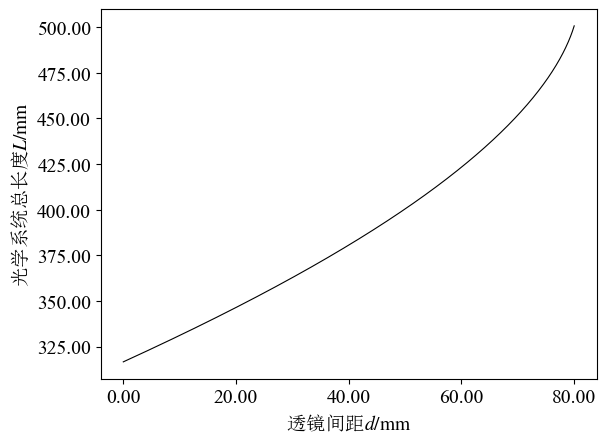
\includegraphics[width=0.8\textwidth]{光学设计,改变总长,d-L.png}
  \caption{改变总长度$L$情况下的组合透镜参数变化情况}
  \label{fig:改变总长,l_2'和l_{H_2}'}
\end{figure}
\par
可见,当透镜的间距增加,系统的总长度将会以更快的速度增长,从而对整体结构造成不利影响,从最小尺寸出发,选取两个透镜的间距为0,即两透镜密接,解得:
\begin{align*}
  \left\{
  \begin{aligned}
    l_H'        & =209.46\unit{\mm}  \\
    l_{H_2}'    & =254.99\unit{\mm}  \\
    l_2'        & =61.61\unit{\mm}   \\
    L           & =316.57\unit{\mm } \\
    l_{H_2H_2'} & =0\unit{\mm}
  \end{aligned}
  \right.
\end{align*}
\par
可见,即使选用最小的尺寸进行设计,得到的光学系统体积仍然较为庞大,这主要是受限于系统的口径和焦距要求。因此,基本的参数设计已经完成,下面检验其孔径和视场要求,并根据这两个要求进一步修改参数,以实现符合实际要求的最佳方案。
\subsection{孔径参数检验}
下面检验其通光口径仍然为$107.14\unit{\mm}$。取靠近照相物镜的一个放大镜,将其当作孔径光阑在经过照相物镜所成像,反求此光阑:
\begin{align*}
  -\frac{1}{l_1}+\frac{1}{l_1'}=\frac{1}{f_1'}
\end{align*}
这里的$l_1'=-l_{H}+l_{H_2}'=45.53\unit{\mm}$,解得:$l_1=49.26\unit{\mm}$,说明孔径光阑位于照相物镜的右侧,再求其通光口径,其中垂轴放大率为$\displaystyle\beta=-\frac{l'}{l}=0.924$,则孔径光阑的口径为$\displaystyle D=\frac{D'}{\beta}=\frac{107.14}{0.924}=115.94\unit{\mm}$,可见变得更大了,同理对下一个放大镜进行相同的操作,得到的光阑口径也变得更大,而光学系统真实的孔径光阑是由通光口径最小的孔径光阑决定的,因此本系统的口径光阑仍然是照相物镜口径$107.14\unit{\mm}$,成像光束口径不受组合透镜影响。\par
对$8\sim14\unit{\um}$波长范围内的辐亮度进行积分,由于辐射体可以看作朗伯体,且距离较远,其立体角可以近似计算为$\displaystyle\Delta\omega=\frac{\alpha\times\beta}{4\pi L_c^2}=1.194\times10^{-7}\unit{sr}$。参考讲义\cite*{hand_up},根据朗伯面辐射体在微面元上的辐照度公式:
\begin{align*}
  {\rm d }E(\lambda)=L_O(\lambda)\cos\varpsi\cdot{\rm d }\omega
\end{align*}
\par
式中,$\varpsi$是辐射体中心对面元法线的方位角,这里取轴向对准目标,因此为0;${\rm d}\omega$是辐射体面元的立体角。对波段内积分,即可得到有效的辐照度,即:
\begin{align*}
  E=\int_{8\unit{\um}}^{14\unit{\um}}L_O(\lambda)\Delta\omega{\rm d}\lambda=3.741\unit{\uW\cdot\m^{-2}}
\end{align*}
\par
上式乘以入瞳面积$\displaystyle\frac{1}{4}\pi D^2$可得入射辐射能。
\subsection{视场参数检验}
验证视场要求:首先进行光路追迹,以确定视场角允许值,带有透镜间距的光学系统光路追迹图如下图\ref{fig:追迹光线确定视场角大小}示:
\begin{figure}[H]
  \centering
  \begin{tikzpicture}
    \coordinate (O) at (0,0);
    \coordinate (A) at (14,0);
    %三个透镜的光心
    \coordinate [label=below:$H_1$] (F1) at (3,0);
    \coordinate [label=below:$H_2$](F2) at (7,0);
    \coordinate [label=below:$H_3$](F3) at (10,0);
    %CCD屏的左端点
    \coordinate [label=below:成像芯片](CCD) at (12,-1);
    %主光轴
    \draw [-{Stealth}] (O) -- (A);
    %画照相系统
    \draw[] (F1) ellipse [x radius=0.2cm,y radius=2cm];
    %放大系统
    \draw[] (F2) ellipse [x radius=0.2cm,y radius=2cm];
    \draw[] (F3) ellipse [x radius=0.2cm,y radius=2cm];
    %CCD
    \draw (CCD) rectangle (12.4,1) ;
    %光学参数
    \coordinate [label=below:$F_1'$] (F1_r) at (13,0);
    \coordinate [label=below:$F_2$] (F2_l) at (5,0);
    \coordinate [label=above:$F_2'$] (F2_r) at (9,0);
    \coordinate [label=below:$F_3$] (F3_l) at (8,0);
    \coordinate [label=above:$F_3'$] (F3_r) at (12,0);
    \filldraw (F1_r) circle [radius=0.6mm];
    \filldraw (F2_r) circle [radius=0.6mm];
    \filldraw (F2_l) circle [radius=0.6mm];
    \filldraw (F3_l) circle [radius=0.6mm];
    \filldraw (F3_r) circle [radius=0.6mm];
    %画一个光路
    %物方
    \draw[line width=0.8pt,red](0,1.8)-- (3,1.5)--(7,0.5)--(10,-1)--(12,-1);
    \draw[line width=0.8pt,arrows = {-Stealth[inset=0pt, length=10pt, angle'=30]},red](3,1.5)--(5,1);
    \filldraw [red] (12,-1) circle [radius=0.6mm];
    %角度标注
    \begin{scope}[>={Stealth[inset=0pt, length=3pt, angle'=30]}]
      \draw[line width=0.4pt](0,1.5)--(3,1.5);
      \path (0,1.8) coordinate (A) --(3,1.5)coordinate(B)--(0,1.5)coordinate(C)
      pic ["$\omega$",draw, line width=0.4pt,angle radius=2cm,angle eccentricity=1.1,<-] {angle = A--B--C};
    \end{scope}
  \end{tikzpicture}
  \caption{追迹光线确定视场角大小}
  \label{fig:追迹光线确定视场角大小}
\end{figure}
\par
特别地,当两组合透镜密接时,光路简化为下图:
\begin{figure}[H]
  \centering
  \begin{tikzpicture}
    \coordinate (O) at (0,0);
    \coordinate (A) at (14,0);
    %三个透镜的光心
    \coordinate [label=below:$H_1$] (F1) at (3,0);
    \coordinate [label=below:$H_2$](F2) at (6.8,0);
    \coordinate [label=below:$H_3$](F3) at (7.2,0);
    %CCD屏的左端点
    \coordinate [label=below:成像芯片](CCD) at (12,-1);
    %主光轴
    \draw [-{Stealth}] (O) -- (A);
    %画照相系统
    \draw[] (F1) ellipse [x radius=0.2cm,y radius=2cm];
    %放大系统
    \draw[] (F2) ellipse [x radius=0.2cm,y radius=2cm];
    \draw[] (F3) ellipse [x radius=0.2cm,y radius=2cm];
    %CCD
    \draw (CCD) rectangle (12.4,1) ;
    %光学参数
    \coordinate [label=below:$F_1'$] (F1_r) at (13,0);
    \coordinate [label=above:$F_2$] (F2_l) at (5,0);
    \coordinate [label=above:$F_2'$] (F2_r) at (9,0);
    \coordinate [label=below:$F_3$] (F3_l) at (5,0);
    \coordinate [label=below:$F_3'$] (F3_r) at (9,0);
    \filldraw (F1_r) circle [radius=0.6mm];
    \filldraw (F2_r) circle [radius=0.6mm];
    \filldraw (F2_l) circle [radius=0.6mm];
    \filldraw (F3_l) circle [radius=0.6mm];
    \filldraw (F3_r) circle [radius=0.6mm];
    %画一个光路
    %物方
    \draw[line width=0.8pt,red](0,2.2)-- (3,1)--(7,-1)--(12,-1);
    \draw[line width=0.8pt,arrows = {-Stealth[inset=0pt, length=10pt, angle'=30]},red](3,1)--(5,0);
    \filldraw [red] (12,-1) circle [radius=0.6mm];
    %角度、线度标注
    \begin{scope}[>={Stealth[inset=0pt, length=5pt, angle'=30]}]
      \draw[|<->|] (3,2.2) --node[above]{$l_x$} (6.8,2.2);
      \draw[line width=0.4pt](0,1)--(3,1);
      \path (0,2.2) coordinate (A) --(3,1)coordinate(B)--(0,1)coordinate(C)
      pic ["$\omega$",draw, line width=0.4pt,angle radius=1cm,angle eccentricity=1.3,<-] {angle = A--B--C};
      \draw[<->] (2,1) --node[left]{$h_1$} (2,0);
      \draw[<->] (11,0) --node[left]{$h_2$} (11,-1);
    \end{scope}
  \end{tikzpicture}
  \caption{追迹光线确定视场角大小}
  \label{fig:追迹光线确定视场角大小,密接}
\end{figure}
\par
从成像芯片的边缘处发出一条平行主光轴的光线,利用光路可逆的原理,反推得到入射光线及临界视场角$\omega$,如果使用简化的模型,即两透镜密切接触,其等效焦距$f_2'=75\unit{\mm}$,则可以按下列各式解算投影高度:
\begin{align*}
  -\frac{1}{\Lambda_2}+\frac{1}{\Lambda_2'}=\frac{1}{f_2'},\Lambda_2'=l_{H_2}'-f' & =147.85\unit{\mm}   \implies \Lambda_2=-152.21\unit{\mm} \\
  h_2=\frac{480}{2}\times                                                         & 12=2.88\unit{\mm}   \quad\text{以最短视场限制计算}                \\
  h_1=\frac{h_2}{l_{H_2}'-\Lambda_2'}=\frac{2.88}{107.14}                         & \times147.85=3.974\unit{\mm}
\end{align*}
\par
入射的视场角为:
\begin{align*}
  \omega=\arctan\frac{h_1}{-\Lambda_2}=\arctan\frac{3.974}{152.21}=1.496^{\circ}
\end{align*}
可见允许的最大视场角$\displaystyle\omega=1.496^{\circ}>\arctan\frac{2}{2000}=0.057^{\circ}$,系统的视场满足题目设计要求。

\newpage
\printbibliography[heading=bibliography,title=参考文献]
\end{document}
